\documentclass[../lab2.tex]{subfiles}

\begin{document}

    \begin{wrapfigure}{r}{0.5\textwidth}
        \centering
        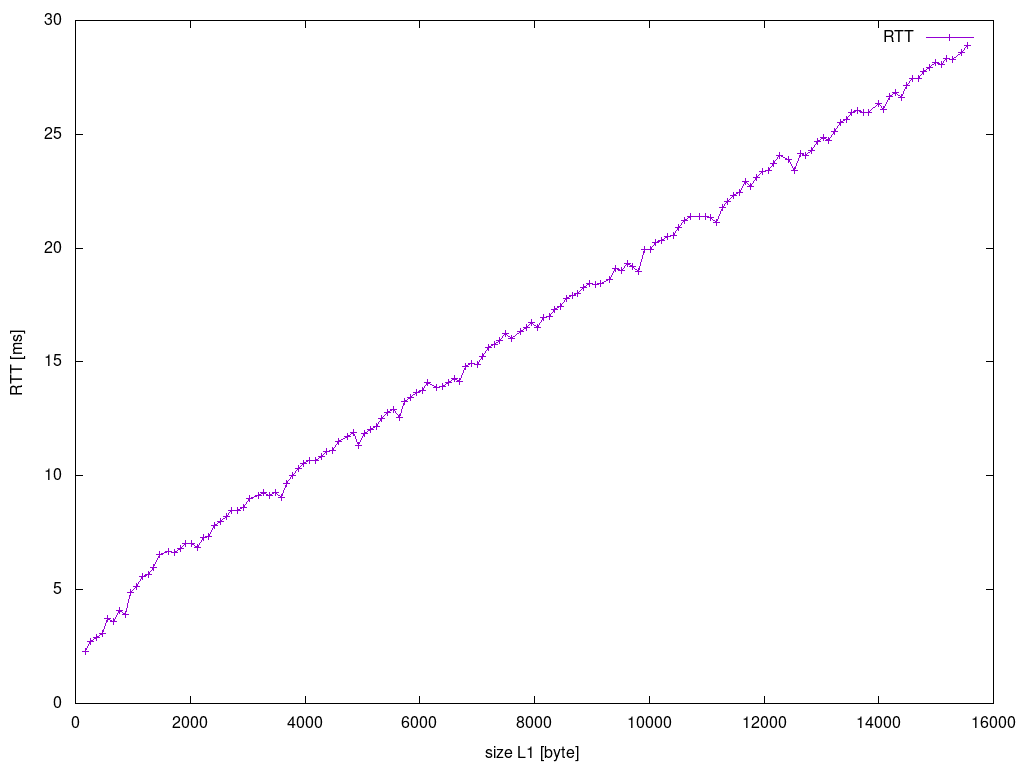
\includegraphics[width=0.5\textwidth]{RTTSetup01.png}
        \vspace{-15pt}
        \caption{RTT}\label{Fig:data1}
    \end{wrapfigure}

            IL grafico riporta l'andamento dell'RTT in funzione dell'aumento
            della dimensione dei pacchetti.
            Si puo' notare una crescita lineare in accordo con quanto ricavato 
            analiticamente, ovvero:

            \begin{equation}
                \centering
                \begin{cases}
                    RTT = 4T_{TX} \qquad \qquad \qquad \, \, D < 1500 \\
                    RTT = 2T_{TX} + 2T_{MTU} \qquad D > 1500
                \end{cases}
            \end{equation}

            \begin{equation}
                \centering
                T_{MTU} = \frac{1538}{V_{TX}}
            \end{equation}

            \begin{equation}
                \centering
                T_{TX} = \frac{D(s)}{V_{TX}}
            \end{equation}

            \begin{equation}
                \centering
                RTT = \frac{2D}{V_{TX2}} +\frac{2D}{V_{TX1}} + T_\eta 
            \end{equation}

            \vspace{30pt}

            Dove $V_{TX1}$ rappresenta la velocita' tra USB/ETH e il router,
            mentre $V_{TX2}$ la velocita' tra PC Live Linux e router.
            $T_\eta$ rappresenta i ritardi propagazione e elaborazione ed e' quasi 
            sempre da considerarsi trascurabile. Nel nostro caso e' un
            valore compreso tra 2 e 3 millisecondi poiche' equivale al valore in X=0
            del grafico RTT. 

    \begin{figure}[!htb]
        \begin{minipage}{0.35\textwidth}
            A partire dagli stessi dati e' possbile ricavare l'effettiva velocita' di 
            trasmissione della rete, considerando i contributi della frammentazione
            come indicato nella formula (2). \\
            Come ci aspettavamo tende asintoticamente 
            a 10Mb/s ossia la velocita' settata inizialemente per la comunicazione tra
            PC Linux Live e router.
        
        \end{minipage}\hfill
        \begin{minipage}{0.6\textwidth}
            \centering
            \includegraphics[width=1\linewidth]{VTxsetup01.png}
            \vspace{-20pt}
            \caption{VTx}\label{VTxsetup01}
        \end{minipage}
    \end{figure}

\end{document}